\chapter{Biological background}
\label{chap:biobackground}

\section{Central dogma of molecular biology}
Proteins are key components within all the organisms in the nature. They perform many important functions such as catalyzing metabolic reactions, DNA replication, responding to stimuli, and transporting molecules from one location to another. The proteins first discovered in 1838 by a Dutch chemist. The process of proteins creation, their functions and their characteristics are an important subject for many studies during the last century. 

In 1958 Francis Crick stated the Central Dogma of Molecular Biology \cite{CRICK1970}, which explains the steps for generating proteins and how they receive their characteristics and functions. The common belief before publishing the dogma was that the protein get their characteristics by an inheritance process. 
The dogma is a framework for understanding the transfer of sequence information between the DNA, the RNA and proteins. 


\section{DNA, RNA and Protein Structures}
Deoxyribonucleic acid (DNA) was first discovered and isolated by Friedrich Miescher in 1869, but it remained understudied for many decades because proteins, rather than DNA, were thought to hold the genetic blueprint to life. This situation changed after 1944 as a result of some experiments by Oswald Avery, Colin MacLeod, and Maclyn McCarty demonstrating that purified DNA could change one strain of bacteria into another. This was the first time that DNA was shown capable of transforming the properties of cells.

In 1953, James Watson and Francis Crick put forward their double-helix model of DNA, based on crystallized X-ray structures being studied by Rosalind Franklin. According to the model, DNA is composed of two strands of nucleotides coiled around each other, linked together by hydrogen bonds and running in opposite directions. 

\subsection{DNA structure}
Each DNA molecule in the cell nucleus consists of two strands of sugars and phosphates with pairs of nitrogen bases forming cross links (Figure \ref{fig:dna_strcture}). This structure is twisted in a spiral shape, called a double helix. To put in basic terms, DNA is two strands coiled together, with chemical cross-links between the two strands. Each Phosphate group and sugar molecule with a nitrogen base attached is called a nucleotide, these are the units that make up the DNA molecule. There are four different types of nitrogen bases, and will only pair in a particular way: 
Adenine (A) will only pair with Thymine (T), and Cytosine (C) will only pair with Guanine (G). The order in which the bases occur in the DNA molecule determines the genetic code. Each gene consists of up to 1000 pairs of bases, this means the number of possible combinations is endless. The subtle structural difference between the sugars gives DNA added stability, making DNA more suitable for storage of genetic information.

\begin{figure}[h!]
	  \centering
	      	\caption{\textbf{DNA structure}}
	      	\label{fig:dna_strcture}

    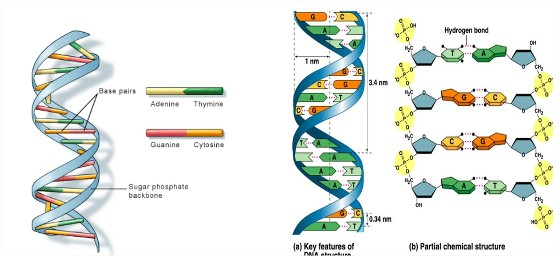
\includegraphics[width=0.5\textwidth]{background figures/dnastructure.jpg}
    	\caption*{The structure of DNA \cite{figDNAStructure}}
    	
    % 	\\Source: \url{https://geneticshbdanieldelprete.weebly.com/structure-of-dna.html}}
\end{figure}

\subsection{RNA Structure}
RNA is typically single stranded and is made of ribonucleotides that are linked by phosphodiester bonds. A ribonucleotide in the RNA chain contains ribose (the pentose sugar), one of the four nitrogenous bases (A, U, G, and C), and a phosphate group (Figure \ref{fig:rna_strcture}). The RNA is relatively instable, which makes it more suitable for its more short-term functions. The RNA-specific pyrimidine uracil forms a complementary base pair with adenine and is used instead of the thymine used in DNA. Even though RNA is single stranded, most types of RNA molecules show extensive intramolecular base pairing between complementary sequences within the RNA strand, creating a predictable three-dimensional structure essential for their function.

\begin{figure}[h!]
	  \centering
	  	\caption{\textbf{RNA structure}}
	  \label{fig:rna_strcture}

    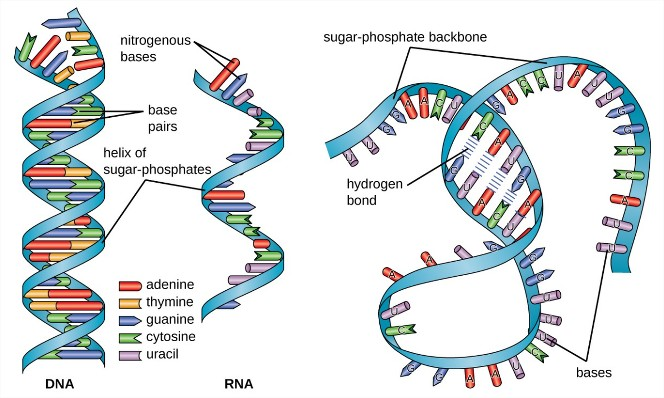
\includegraphics[width=0.5\textwidth]{background figures/rnastructure.jpg}
    	\caption*{The structure of RNA.\\  RNA can fold upon itself, with the folds stabilized by short areas of complementary base pairing within the molecule, forming a three-dimensional structure.\cite{figRNAStructure}
    	}
    % 	\url{https://courses.lumenlearning.com/microbiology/chapter/structure-and-function-of-rna}}
\end{figure}

\subsection{Protein Structure}
Proteins are large, complex molecules that are critical for the normal functioning of the human body. They are essential for the structure, function, and regulation of the body's tissues and organs. Proteins are made up of hundreds of smaller units called amino acids that are attached to one another by peptide bonds, forming a long chain (Figure \ref{fig:protein_structure}).
The four levels of protein structure are: primary structure, secondary structure, tertiary structure, and quaternary structure. 

\begin{figure}[h!]
	  \centering
	  \caption{\textbf{The structure of Protein}}
	  	  \label{fig:protein_structure}


    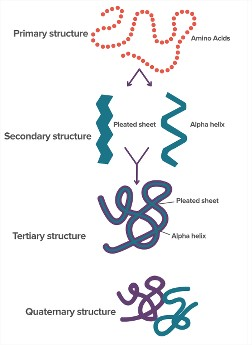
\includegraphics[width=0.5\textwidth]{background figures/proteinstructure.jpg}
    	\caption*{The structure of Protein.\cite{figProteinStructure}
    	}
    % 	\\ Source: \url{https://www.khanacademy.org/test-prep/mcat/biomolecules/amino-acids-and-proteins1/a/chemistry-of-amino-acids-and-protein-structure}}
\end{figure}

\section{Transferring information between DNA, RNA and protein}
The DNA and the RNA are both nucleic acids. The DNA carries the genetic instructions for major process of all the living organisms including growth, development, functioning and reproduction. The RNA is responsible of coding, decoding, regulation and expression of the genes.
There are 9 theoretical combinations to transfer information between pairs of DNA, RNA and protein. The dogma (central dogma of molecular biology) classes the combinations into 3 classes as shown in Table\ref{table:1}

\begin{table}[h!]
\centering
\begin{tabular}{||c c c ||} 
\hline
	General & Special & Unknown \\ \hline
	DNA $\rightarrow$ DNA & RNA $\rightarrow$ DNA & Protein $\rightarrow$ DNA \\ \hline
	DNA $\rightarrow$ RNA & RNA $\rightarrow$ RNA & Protein $\rightarrow$ RNA \\ \hline
   	RNA $\rightarrow$ Protein & DNA $\rightarrow$ Protein & Protein $\rightarrow$ Protein \\ \hline
\end{tabular}
\caption{Three classes of information transfer. The popular assumption focused on the “General” column.}
\label{table:1}
\end{table}

In the past three decades, the popular assumption focused on the “General” column of the table and stated that the generation of a protein consists of two steps: the first step is DNA  to RNA interaction and the second step is RNA to protein interaction (Figure \ref{fig:infoflowbio}). A major part of the assumption was that the RNA molecule has only coding areas and all of it is translated into the protein.

\begin{figure}[h!]
	  \centering
	  \caption{\textbf{Information flow in biological systems}}
	  	  \label{fig:infoflowbio}

    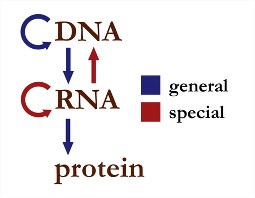
\includegraphics[width=0.3\textwidth]{background figures/dna2rna2protein.jpg}
    	\caption*{Information flow diagram. \cite{figRnaDnaPro}
    	}
    % 	\\ Source: \url{https://en.wikipedia.org/wiki/Central_dogma_of_molecular_biology}}
\end{figure}

\section{Non-coding RNA}
A non-coding RNA (ncRNA) is an RNA molecule that is not translated into a protein. These RNAs appear to comprise a hidden layer of internal signals that control various levels of gene expression in physiology and development, including chromatin architecture/epigenetic memory, transcription, RNA splicing, editing, translation and turnover. RNA regulatory networks may determine most of our complex characteristics, play a significant role in disease and constitute an unexplored world of genetic variation both within and between species. \\
Emerging evidence from the human genome sequencing projects suggests that more than 80\% of the human genome is actively transcribed into RNA, even though less than 3\% of the human genome encodes translated proteins \cite{Consortium2012}. RNAs that do not yield coding proteins are collectively referred to as non-coding RNAs (ncRNA). These ncRNAs are divided into housekeeping ncRNAs and regulatory ncRNAs. Housekeeping ncRNAs include transfer RNAs (tRNAs) and ribosomal RNAs (rRNAs). Regulatory ncRNAs are generally transcribed in a location- and time-dependent fashion. Regulatory ncRNAs can be further divided into two groups based on their size: small ncRNAs (shorter than 200 nucleotides) and lncRNAs (200 nucleotides or longer). Small ncRNAs contain microRNAs, small nucleolar RNAs (snoRNAs), small interfering RNAs (siRNAs), small nuclear RNAs (snRNAs), and PIWI-interacting RNAs (piRNAs). For full diagram, see Figure \ref{fig:rnacategories}.

\begin{figure}[h!]
	  \centering
	      	\caption{\textbf{RNA categories}}
	  \label{fig:rnacategories}

  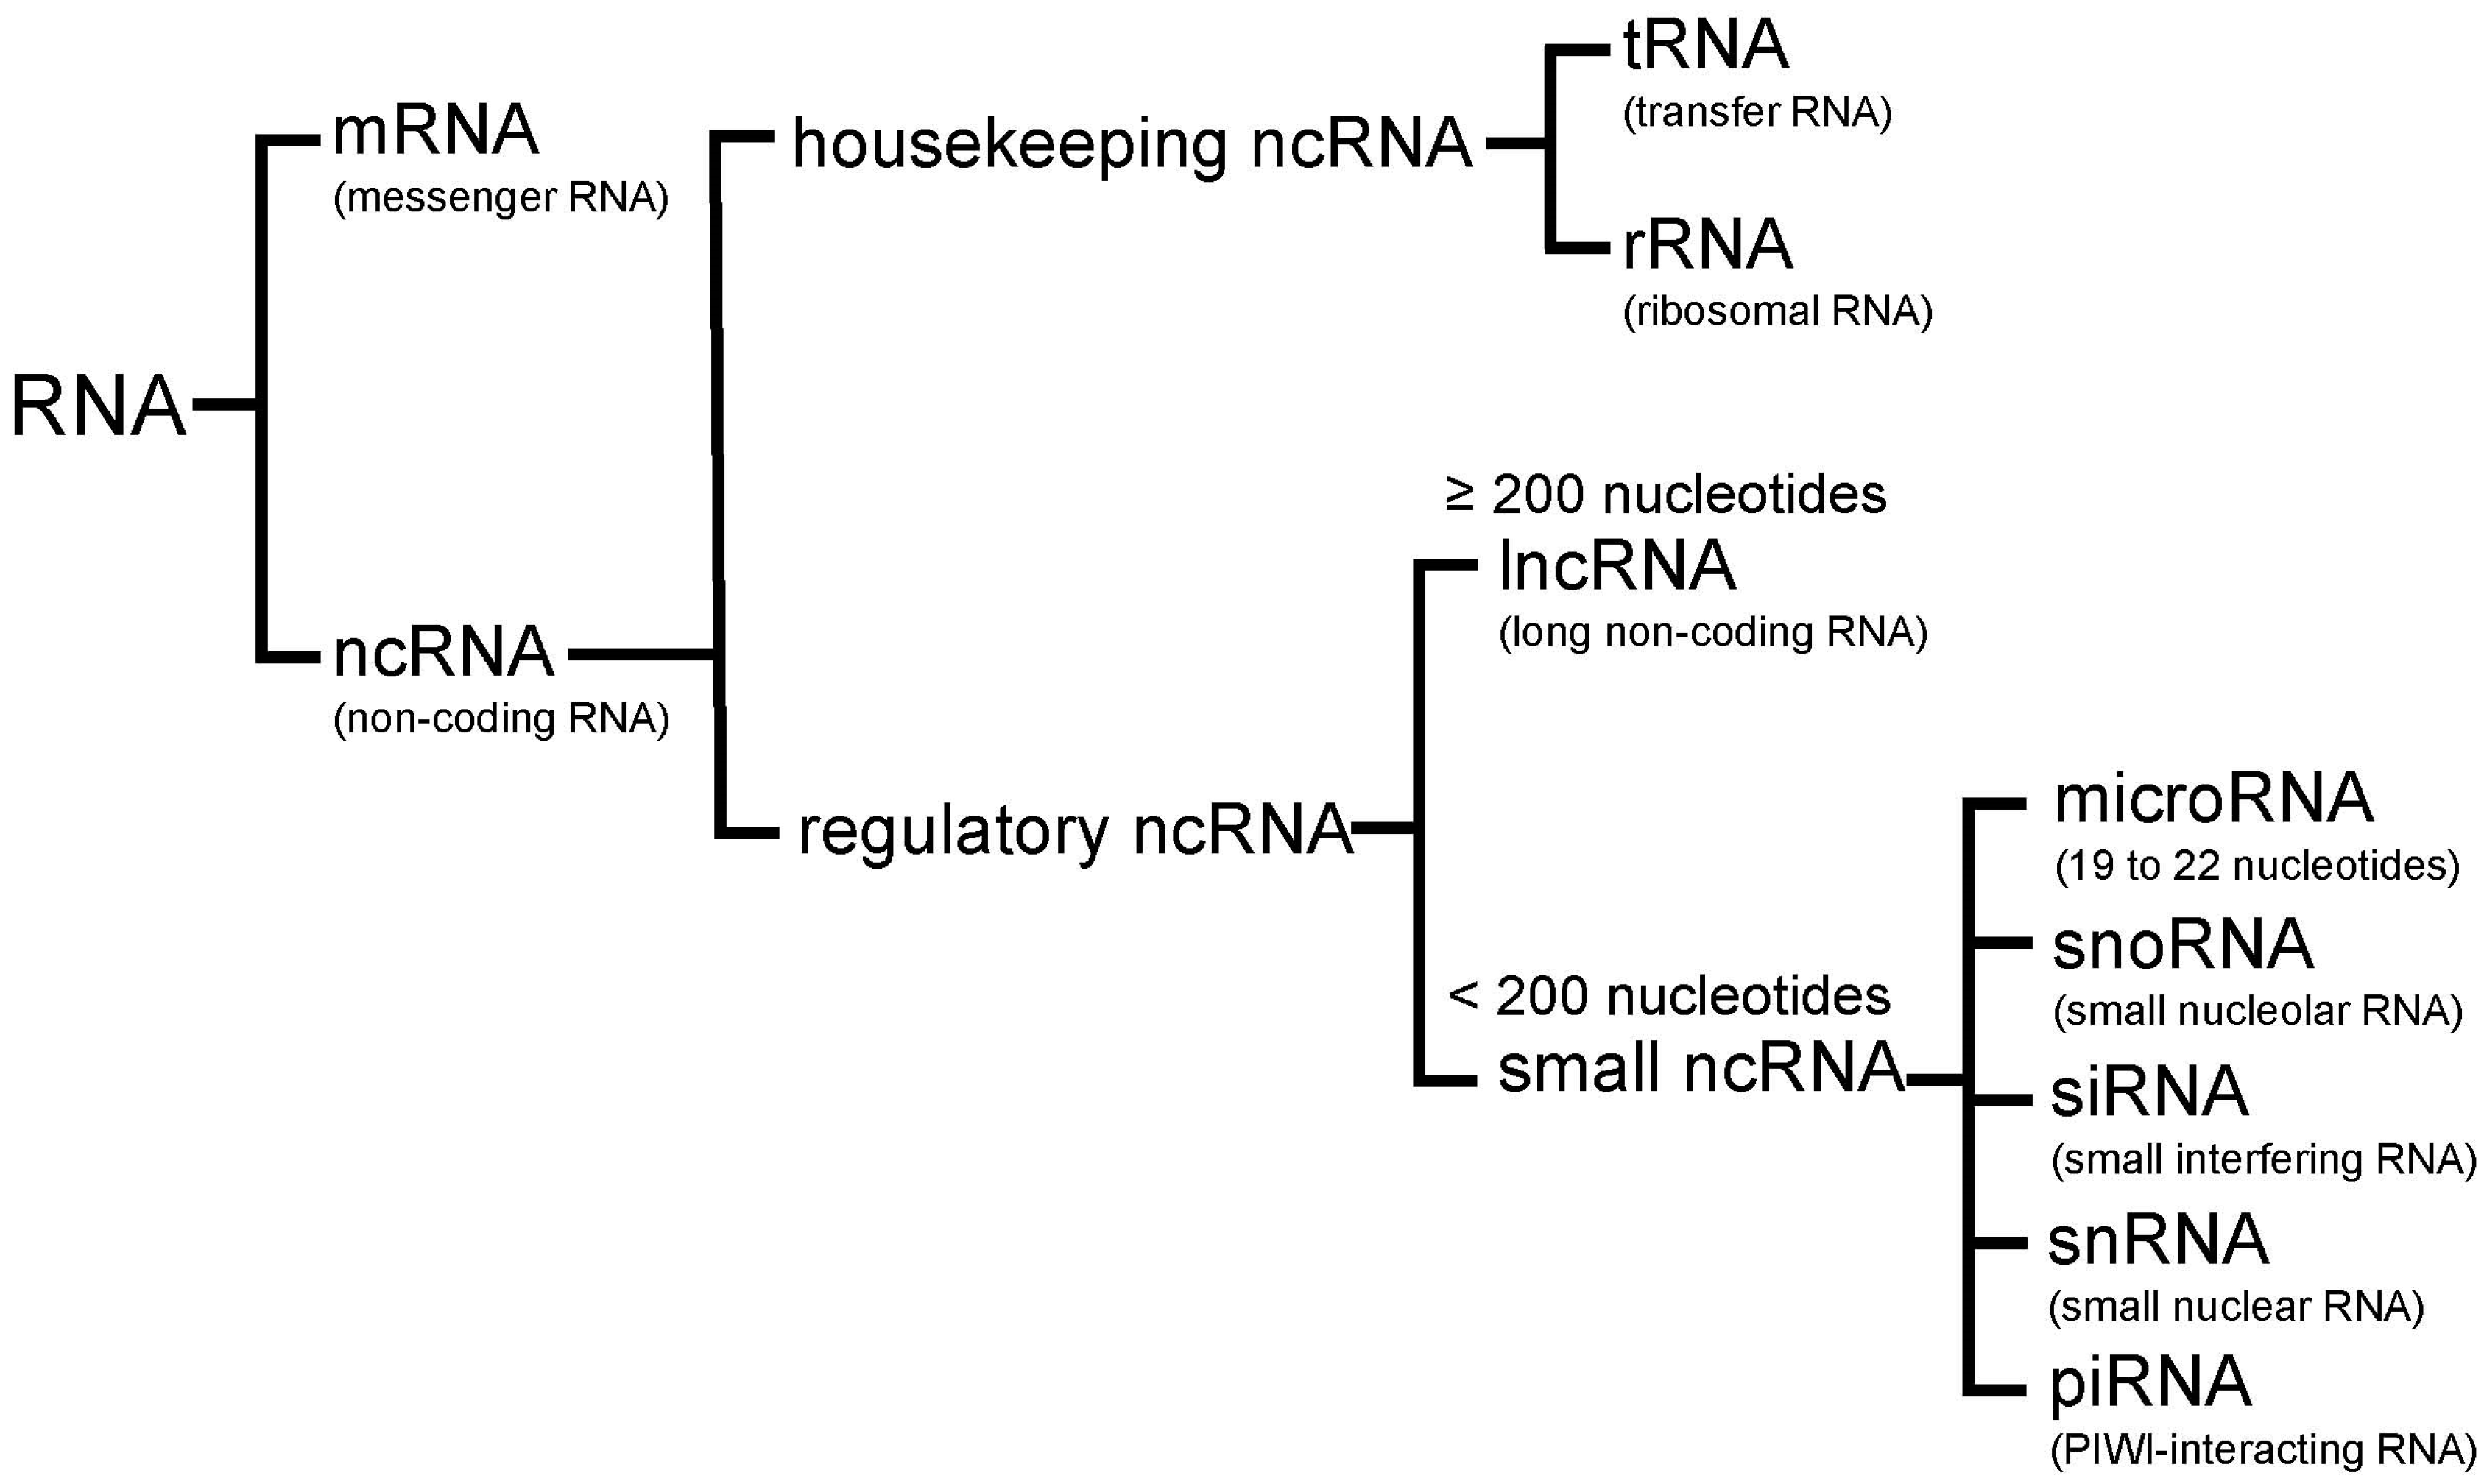
\includegraphics[width=0.5\textwidth]{background figures/cells-06-00012-g001.png}
    	\caption*{Source: \cite{Inamura2017}}
  
\end{figure}

\section{MicroRNA (MiRNA)}

It has been generally assumed that most genetic information is transacted by proteins. In \textit{1993}, \textit{Rosalind C. Lee, Rhonda L. Feinbaum and Victor Ambros} published the article \textit{The C. elegans heterochronic gene lin-4 encodes small RNAs with antisense complementarity to lin-14} \cite{LEE1993843}. It described the discovery of post-transcriptional gene silencing by antisense RNA–RNA interaction in nematodes, introducing a new mechanism of gene expression regulation in metazoan. Later on, more evidence suggests that the majority of the genomes of mammals and other complex organisms is in fact transcribed into Non-coding RNA (ncRNAs). \\
MicroRNAs (miRNAs) are small non-coding RNA molecules (containing about 22 nucleotides) found in plants, animals and some viruses, that functions in RNA silencing and post-transcriptional regulation of gene expression. In humans and other mammals, these small RNAs help control the expression of most mRNAs. Recent studies suggest that miRNAs influence essentially all developmental process and diseases \cite{mirbase1}. Indeed, loss-of-function studies disrupting miRNA genes in mice have revealed diverse phenotypes, including defects in the development of the skeleton, teeth, brain, eyes, neurons, muscle, heart, lungs, kidneys, vasculature, liver, pancreas, intestine, skin, fat, breast, ovaries, testes, placenta, thymus, and each hematopoietic lineage, as well as cellular, physiological, and behavioral defects. Many of these developmental and physiological defects affect embryonic or postnatal viability or cause other severe conditions, such as epilepsy, deafness, retinal degeneration, infertility, immune disorders, or cancer. In addition, some miRNA knockout strains have altered susceptibility to infections, and many have differential responses to mouse models of diseases
or injuries \cite{Bartel2018}.

\subsection{MiRNA Biogenesis}
miRNA genes are mainly transcribed by RNA polymerase II, producing a primary (pri)-miRNA that is capped, polyadenylated, and spliced (Figure \ref{fig:miRNAprocessingpathway}). The processing of miRNA genes depends on their secondary structure, and the stable hairpin structure of the pre-miRNA is the clearest characteristic of miRNA transcripts.
\begin{itemize}
\item The majority of miRNA genes are processed in the nucleus by the microprocessor complex consisting of the proteins RNASEN (also known as Drosha). The 50–80-nt Drosha product (pre-miRNA) is exported to the cytoplasm and subsequently processed by the enzyme Dicer. 
\item A minority of the miRNAs, called mirtrons, do not require Drosha processing and instead are produced from intronic hairpins that are formed after splicing of protein-coding genes.
\end{itemize}
After Dicer processing, one of the two arms of the miRNA duplex is loaded into the RNA induced silencing complex (RISC). Incorporation of either of the strands depends on the thermodynamic stability of the 5' region of the miRNA in the duplex. The nonincorporated miRNA* species is subsequently degraded. Targeting of miRNAs to the 3' UTR of mRNAs depends on RISC, which mediates the imperfect base pairing of miRNAs to mRNAs. \\ Nucleotides 2–7 of mature miRNAs, known as the "seed region", are the primary determinants of miRNA target recognition.

\begin{figure}[ht!]
	  \centering
	      	\caption{\textbf{miRNA processing pathway}}
	      		  \label{fig:miRNAprocessingpathway}

    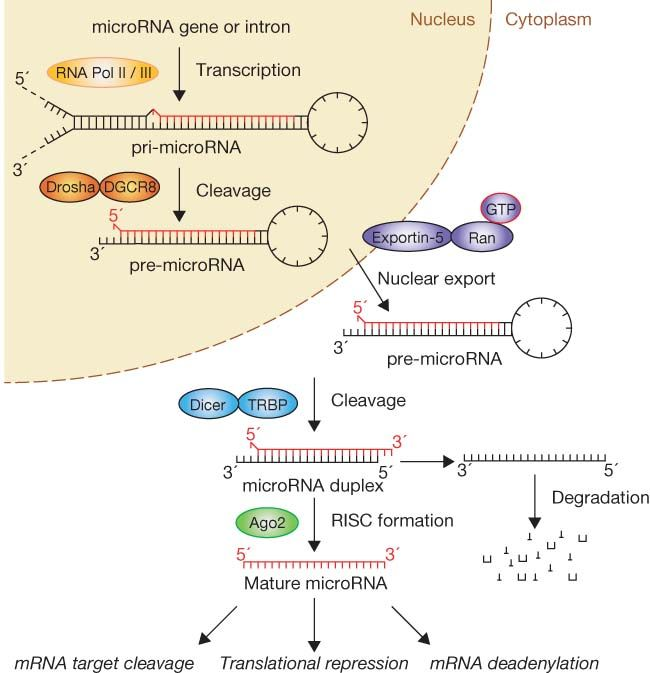
\includegraphics[width=0.5\textwidth]{background figures/ThelinearcanonicalpathwayofmicroRNAprocessing.jpg}
    	\caption*{Source: \cite{Winter2009}}
\end{figure}


\subsection{MiRNA interactions in animals}
Animal microRNAs (miRNAs) pair to 3'UTRs of mRNAs to direct their posttranscriptional repression. Important for target recognition are ~7 nt sites that match the seed region of the miRNA \cite{GRIMSON200791}. More than one-third of human genes appear to have been under selective pressure to maintain their pairing to miRNA seeds \cite {LEWIS200515} and many messages that either decrease upon miRNA ectopic expression or increase upon miRNA knockdown have matches to the miRNA seed \cite{Krutzfeldt2005, Lim2005}.
% (Krutzfeldt et al., 2005, Lim et al., 2005, Giraldez et al., 2006, Rodriguez et al., 2007).

% Messenger RNAs downregulated after introducing a miRNA are most associated with two types of sites:
Nine seed types are categorized in two groups (Figure \ref{fig:mirnaseedtypes}); "Stringent" (8mer, 7mer-A1, and 7mer-m8) and "Non-stringent" (6mer, GUM, GUT, LP, BM and BT). GUM and GUT allow one GU wobble in the seed region. GUM has the U on miRNA whereas GUT has the U on the target. LP, BM and BT allow one mismatch. LP has one loop, BM has one bulge on miRNA, and BT has one bulge on the target.


\begin{figure}[ht!]
	  \centering
	  	\caption{\textbf{miRNA seed types}}
	  	\label{fig:mirnaseedtypes}
    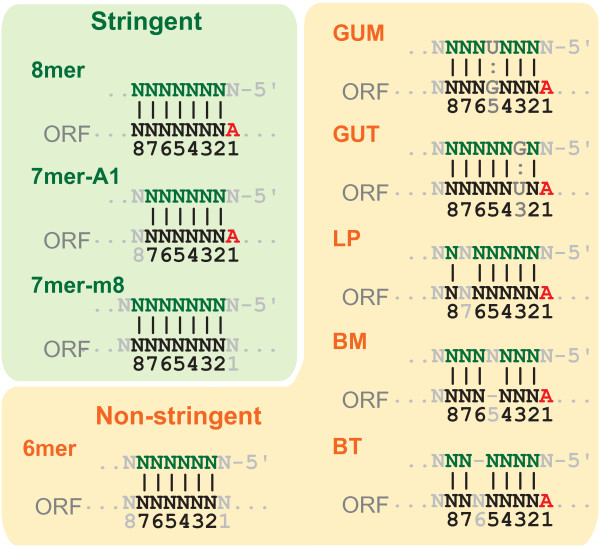
\includegraphics[width=0.5\textwidth]{background figures/miRNA-seed-types-Nine-seed-types-are-categorized-in-two-groups-Stringent-8mer.png}
    	\caption*{Nine seed types are categorized in two groups; "Stringent" and "Non-stringent". \cite{seedarticle}}
\end{figure}



\subsection{Evolution of miRNA genes}
Since their discovery in Caenorhabditis elegans (C. elegans) in 1993 \cite{LEE1993843}, miRNAs   were shown to be present in all animals and plants and in many viruses \cite{mirbase1} (Figure \ref{evo_fig}). Studies have demonstrated that plant and animal miRNAs operate through different mechanisms and show little or no sequence similarity \cite{moran2017evolutionary}, findings that led to the conclusion that miRNAs evolved independently in those distinct lineages.



\begin{figure}[ht!]
	  \centering
	  \caption{\textbf{Phylogenetic distribution of miRNA sequences}}
	    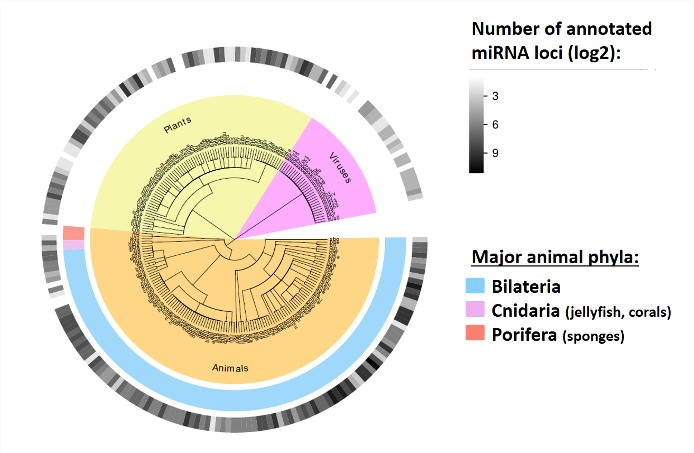
\includegraphics[width=0.5\textwidth]{background figures/evolution.jpg}
    	\caption*{Phylogenetic distribution of miRNA sequences registered in the latest version of miRBase, the main miRNA database \cite{mirbase1}. A phylogenetic tree of 223 species classified into animals, plants and viruses, and their corresponding numbers of miRNA entries (shown in log2 scale).}
    	\label{evo_fig}
\end{figure}


